\chapter{Edge detection}

In this chapter let us focus on the main goal of the thesis, which is edge detection. What is an edge? It is a place where image brightness changes rapidly. There are various methods to identify such discontinuities. The most popular are gradient based (e.g. Canny, Prewitt, Sobel) and Laplacian based. However, there is also another method, which provides similar results and can be more efficient in terms of computation. This method is based on the 2-Dimensional Discrete Wavelet Transform described in section \ref{sec:2D_DWT}. \newline

What should be done? \textit{** Link to article Edge detection **}
\begin{enumerate}
\item Convert image to grey scale.
\item Apply 2-D DWT on an image.
\item Remove the LL part.
\item Denoise the LH, HL and HH coefficients.
\item Reconstruct the initial image.
\item Post-processing - modify contrast to emphasize obtained edges.
\end{enumerate}

\section{Implementation of an algorithm}

The algorithm is implemented in \texttt{Python} using library/package (?) \texttt{PyWavelets}. There are used also auxiliary libraries like: \texttt{numpy}, \texttt{matplotlib}, \texttt{PIL} and \texttt{scipy}. The \texttt{PyWavelets} package contains all features required to edge detection algorithm, i.e. 2D Forward and Inverse Discrete Wavelet Transform, build-in many wavelet functions and thresholding functionality (used to denoise coefficients).

Lets go deeper into algorithm, using a simple example - white square on a black background.

\begin{figure}[h]
	\centering
	
\includegraphics[width=0.3\textwidth]{graphs/square.png}
	\caption{An initial image - a white square.}
\end{figure}

Initially, a colour image must be simplified by conversion to grey scale. Edges are recognised as changes in brightness, so a single pixel should contains only information about a colour (black) intensity. Our initial image is already black and white so we do not need to convert it. Now, we can apply the 2D DWT function. As a result, according to the description in section \ref{sec:2D_DWT}, we obtain four components of wavelet coefficients: LL, LH, HL and HH show on a graph \ref{fig:square_coeffs}. It is clearly visible that the LL part reflects the initial image and the rest components contains information about rapid brightness changes in particular directions. 

\begin{figure}[h]
	\centering
	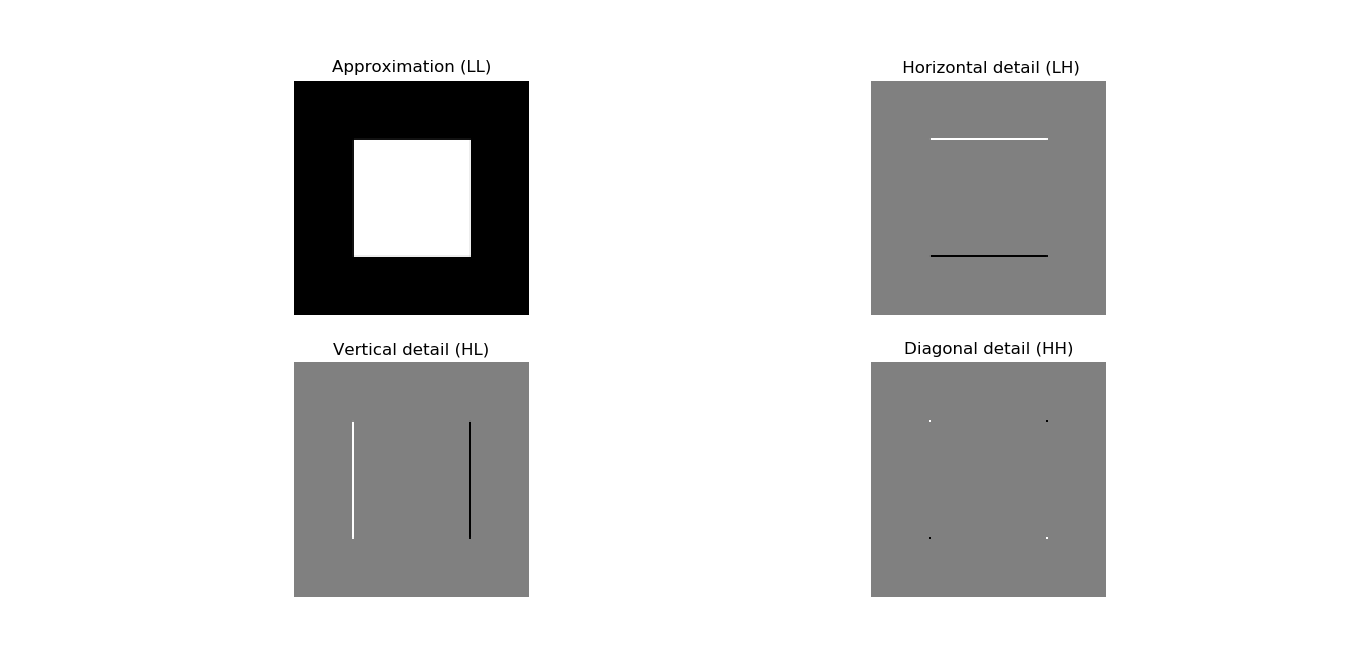
\includegraphics[width=\textwidth]{graphs/square_db2_coeffs.png}
	\caption{2-D DWT coefficients.}
	\label{fig:square_coeffs}
\end{figure}

Thus, we are interested only in components which gives information about edges, so we remove the approximation part - figure \ref{fig:square_coeffs_d}.

\begin{figure}[h]
	\centering
	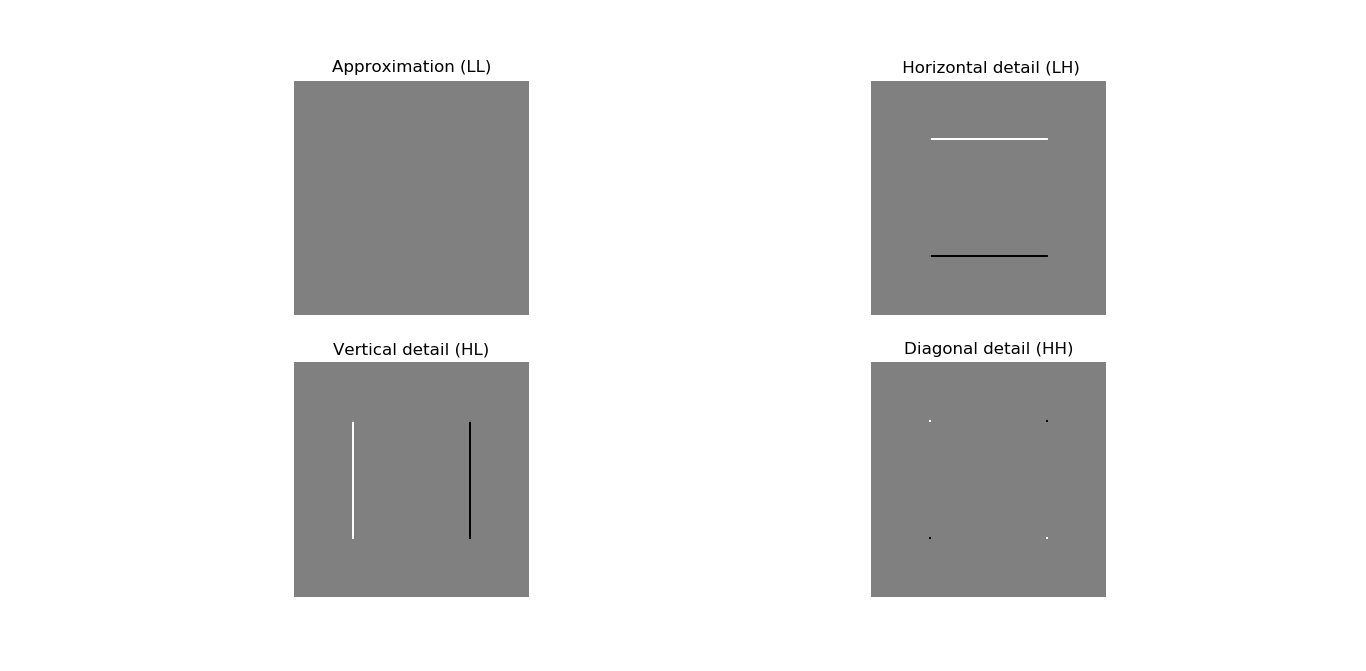
\includegraphics[width=\textwidth]{graphs/square_db2_coeffs_d.png}
	\caption{2-D DWT coefficients with removed the LL part.}
	\label{fig:square_coeffs_d}
\end{figure}

Subsequently, remaining components can be denoised. It means, we can /pozbyc sie/ small, insignificant coefficients by thresholding. More about setting the threshold is described in section \ref{sec:threshold}. This simple example do not require any denoising, so lets go to further.

The last main step is reconstruction of the initial image, i.e. application an inverse 2-D DWT on the denoised coefficients. In the result, we obtain the edges of the initial image presented on a graph \ref{fig:square_idwt}.

\begin{figure}[h]
	\centering
	
\includegraphics[width=0.3\textwidth]{graphs/square_db2.png}
	\caption{A reconstructed image showing the edges.}
	\label{fig:square_idwt}
\end{figure}

At the end, we can do some post-processing to emphasize obtained lines. Currently, a background has grey colour and the edges are white or black. Therefore, using simple mathematical calculations we can modify image to have black background and white edges. It is enough to get an absolute value, subtract 128 and then scale by multiplying 2 times.
\textit{** Add some more about values in an image array, here or in the previous paragraph **}
Finally, we obtain the edges of the square shown on a figure \ref{fig:square_idwt_pp}.

\begin{figure}[h]
	\centering
	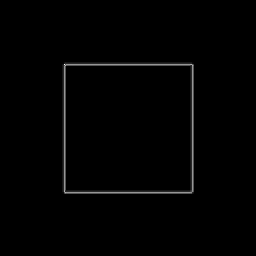
\includegraphics[width=0.3\textwidth]{graphs/square_db2_pp.png}
	\caption{The edges of the square image after post-processing.}
	\label{fig:square_idwt_pp}
\end{figure}

\section{Thresholding}
\label{sec:threshold}
There are two types of thresholding hard and soft. Lets denote $\lambda$ as threshold value and $d$ as wavelet coefficient. The hard one /nadaje/ zero value for coefficients below the set threshold. It is defined as follow

\begin{equation}
D^H(d|\lambda)=
\begin{cases}
0, & \text{for } |d| \leq \lambda, \\
d, & \text{for } |d| > \lambda.
\end{cases}
\end{equation}

While, the soft thresholding works in the same way on the coefficients smaller than $\lambda$, but additionally the coefficient bigger than the set threshold are ''shrinked'' towards zero /o jego wartosc/, as it is defined below.

\begin{equation}
D^S(d|\lambda)=
\begin{cases}
	0, & \text{for } |d| \leq \lambda, \\
	d-\lambda, & \text{for } d > \lambda, \\
	d+\lambda, & \text{for } d < -\lambda.
\end{cases}
\end{equation}


\subsection{Hard or soft thresholding}

To see the differences between both types of thresholding lets consider a noisy image (fig. \ref{fig:square_s10}).

\begin{figure}[h]
	\centering
	
\includegraphics[width=0.3\textwidth]{graphs/square_s10.png}
	\caption{A noisy square image.}
	\label{fig:square_s10}
\end{figure}

The coefficients of 2-D DWT are shown on the graph \ref{fig:square_s10_coeffs}.

\begin{figure}[h]
	\centering
	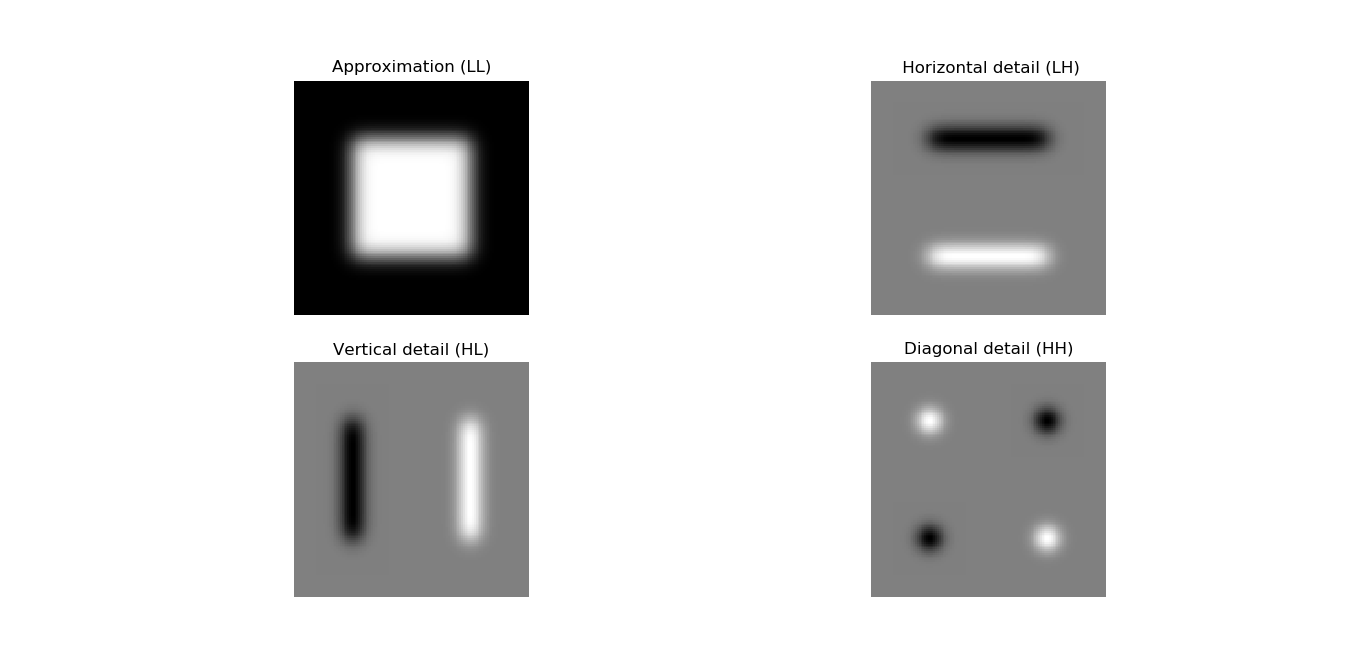
\includegraphics[width=\textwidth]{graphs/square_s10_db1_coeffs.png}
	\caption{2-D DWT coefficients.}
	\label{fig:square_s10_coeffs}
\end{figure}

Now, according to the edge detection algorithm, we remove the LL component and we can denoise the others. Results of hard and soft thresholding are presented respectively on a figures \ref{fig:square_s10_hard_coeffs_d} and \ref{fig:square_s10_soft_coeffs_d}.

\begin{figure}[h]
	\centering
	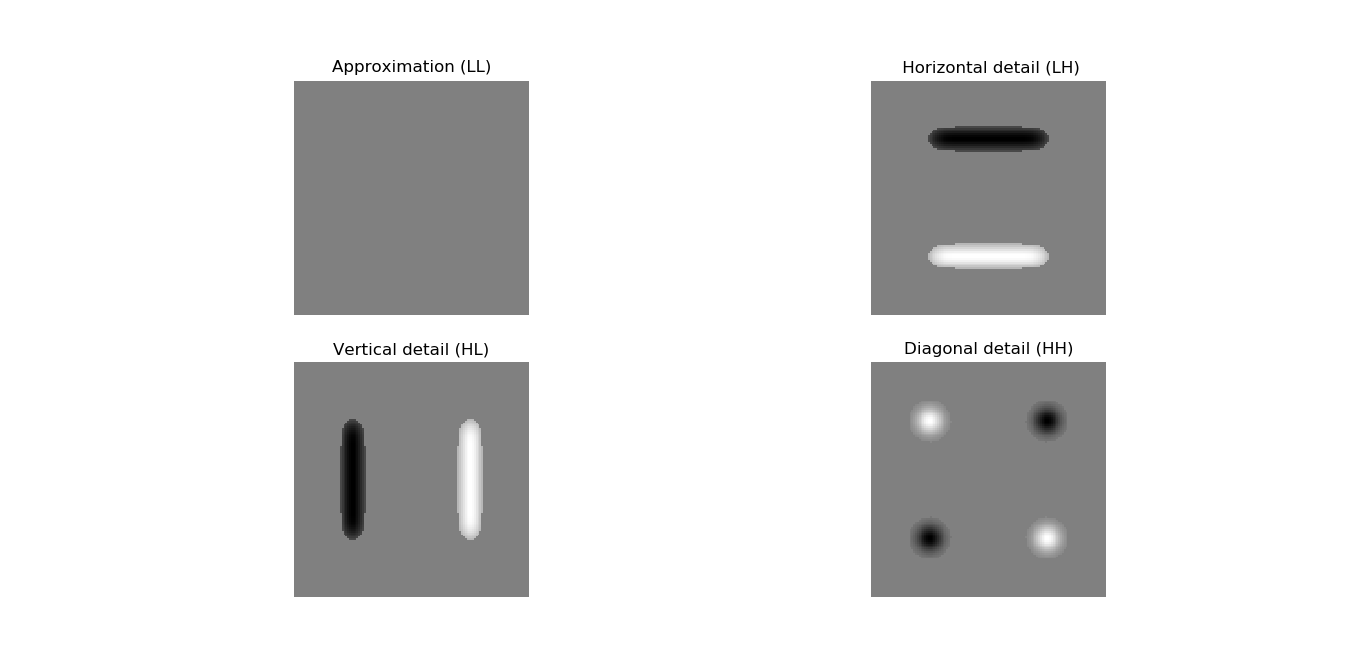
\includegraphics[width=\textwidth]{graphs/square_s10_db1_hard_coeffs_d.png}
	\caption{2-D DWT coefficients after hard thresholding.}
	\label{fig:square_s10_hard_coeffs_d}
\end{figure}

\begin{figure}[h]
	\centering
	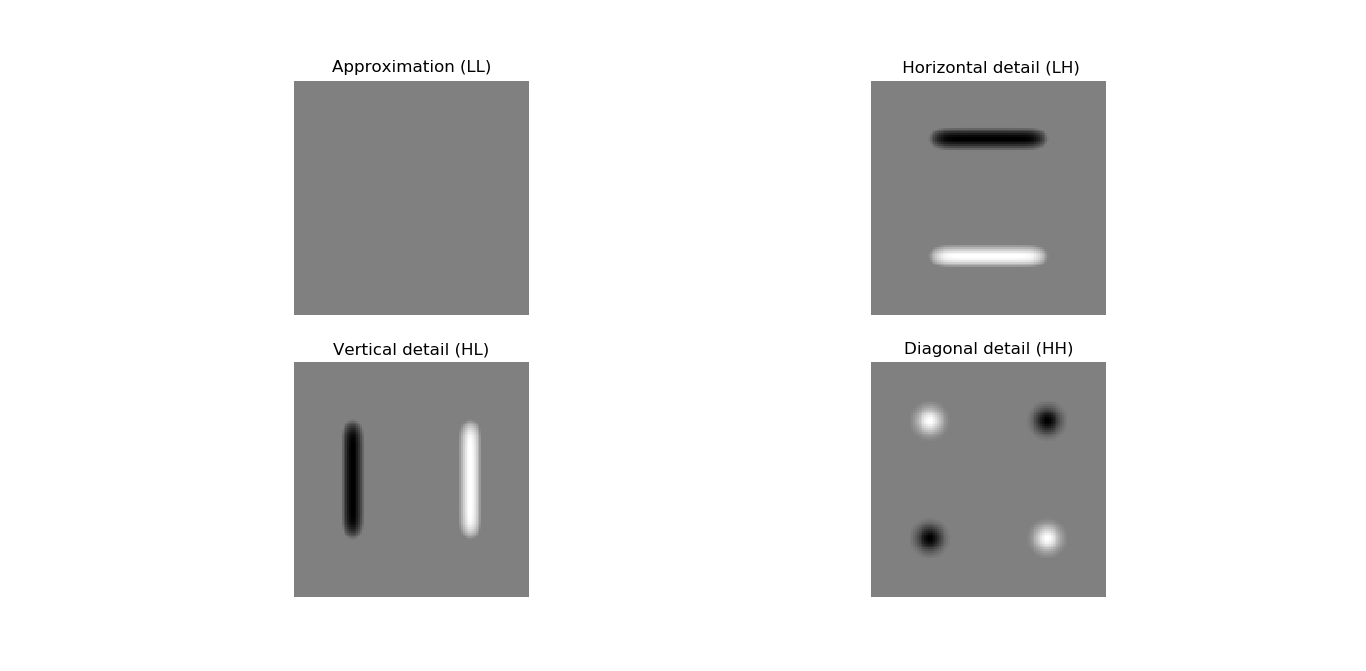
\includegraphics[width=\textwidth]{graphs/square_s10_db1_soft_coeffs_d.png}
	\caption{2-D DWT coefficients after soft thresholding.}
	\label{fig:square_s10_soft_coeffs_d}
\end{figure}

Especially on the LH and HL components we can see the distinction between both thresholding. After soft one the lines are smoother and slightly narrower the in the other case. Therefore, the soft thresholding is better for edge detection (smoother edges are better, /wybacza bledy bardziej niz hard/). To confirm this conclusion lets compare the final results, after inverse DWT (fig. \ref{fig:square_s10_idwt_pp})

\begin{figure}[h]
	\begin{subdiagrams}{square_s10_db1_hard_pp}{square_s10_db1_soft_pp}
	\end{subdiagrams}
	\centering
	\caption{Results of edge detection with hard (a) and soft (b) thresholding.}
	\label{fig:square_s10_idwt_pp}
\end{figure}

\subsection{Selection of the threshold}
The key is how to set the $\lambda$ to denoise coefficients and do not loose any significant information.
\textit{** Some more about it and how I choose the threshold **}

\section{Wavelet types}

\textit{** Show how algorithm work on a simple square **}